% =============================================================================
% КАНОНИЧЕСКИЕ СХЕМЫ УРОКА 2: ЕДИНСТВЕННЫЙ РАБОЧИЙ ИСТОЧНИК
% =============================================================================
% Каждая конфигурация скопирована из текущих исходников Ященко-2022.
% В аргументах макросов допускается менять только числовые подписи.

% Вариант 22: касательный четырёхугольник.
\newcommand{\figTangentialQuad}[3]{%
\begin{tikzpicture}[scale=1.25,line cap=round,line join=round,every node/.style={font=\small}]
  \coordinate (O) at (0,0);
  \coordinate (A) at (-1.462,-0.532); \coordinate (B) at ( 0.598,-1.282);
  \coordinate (C) at ( 1.179, 0.316); \coordinate (D) at (-0.270, 1.532);
  \draw[line width=0.9pt] (A)--(B)--(C)--(D)--cycle;
  \draw[line width=0.9pt] (O) circle (1);
  \path (A)--(B) node[midway,below left] {$#1$};
  \path (B)--(C) node[midway,right=2mm] {$#2$};
  \path (C)--(D) node[midway,above right] {$#3$};
  \node[left] at (A) {$A$}; \node[below] at (B) {$B$};
  \node[right] at (C) {$C$}; \node[above] at (D) {$D$};
\end{tikzpicture}}

% Вариант 13: касательный четырёхугольник и периметр.
\newcommand{\figTangentialPerimeter}{%
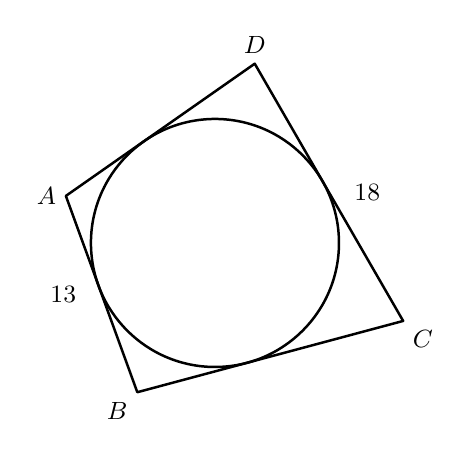
\begin{tikzpicture}[scale=1.05,line cap=round,line join=round,every node/.style={font=\small}]
  \coordinate (O) at (0,0);
  \coordinate (A) at (-1.803, 0.569); \coordinate (B) at (-0.939,-1.805);
  \coordinate (C) at ( 2.276,-0.943); \coordinate (D) at ( 0.481, 2.168);
  \draw[line width=0.9pt] (A)--(B)--(C)--(D)--cycle;
  \draw[line width=0.9pt] (O) circle (1.5);
  \path (A)--(B) node[midway,left=2mm] {$13$};
  \path (C)--(D) node[midway,right=2mm] {$18$};
  \node[left] at (A) {$A$}; \node[below left] at (B) {$B$};
  \node[below right] at (C) {$C$}; \node[above] at (D) {$D$};
\end{tikzpicture}}

% Вариант 5: биссектриса тупого угла параллелограмма.
\newcommand{\figParallelogramBisector}{%
\begin{tikzpicture}[scale=0.72,line cap=round,line join=round,every node/.style={font=\small}]
  \coordinate (A) at (0,0); \coordinate (B) at (7,0); \coordinate (E) at (3,0);
  \coordinate (D) at (0.8,2.891); \coordinate (C) at (7.8,2.891);
  \draw[line width=0.9pt] (A)--(B)--(C)--(D)--cycle;
  \draw[line width=0.9pt] (D)--(E);
  \pic[draw,line width=0.65pt,angle radius=5mm] {angle=A--D--E};
  \pic[draw,line width=0.65pt,angle radius=5mm] {angle=E--D--C};
  \node[below left] at (A) {$A$}; \node[below right] at (B) {$B$};
  \node[above right] at (C) {$C$}; \node[above left] at (D) {$D$}; \node[below] at (E) {$E$};
  \node[below=4mm] at ($(A)!0.5!(E)$) {$3$};
  \node[below=4mm] at ($(E)!0.5!(B)$) {$4$};
\end{tikzpicture}}

% Вариант 6: две биссектрисы параллелограмма.
\newcommand{\figParallelogramTwoBisectors}{%
\begin{tikzpicture}[scale=0.78,line cap=round,line join=round,every node/.style={font=\small}]
  \coordinate (A) at (0,0); \coordinate (B) at (6,0);
  \coordinate (D) at (1,2.828); \coordinate (C) at (7,2.828); \coordinate (E) at (3,0);
  \draw[line width=0.9pt] (A)--(B)--(C)--(D)--cycle;
  \draw[line width=0.9pt] (D)--(E)--(C);
  \pic[draw,line width=0.65pt,angle radius=4.8mm] {angle=A--D--E};
  \pic[draw,line width=0.65pt,angle radius=4.8mm] {angle=E--D--C};
  \pic[draw,line width=0.65pt,angle radius=4.8mm] {angle=D--C--E};
  \pic[draw,line width=0.65pt,angle radius=4.8mm] {angle=E--C--B};
  \node[below left] at (A) {$A$}; \node[below right] at (B) {$B$};
  \node[above right] at (C) {$C$}; \node[above left] at (D) {$D$}; \node[below] at (E) {$E$};
\end{tikzpicture}}

% Вариант 9: ромб с вписанной окружностью. Внутренних точек и перпендикуляра нет.
\newcommand{\figRhombusCircle}[1]{%
\begin{tikzpicture}[scale=0.62,line cap=round,line join=round,every node/.style={font=\small}]
  \coordinate (A) at (0,0); \coordinate (B) at (6,0);
  \coordinate (D) at (5.196,3); \coordinate (C) at (11.196,3); \coordinate (O) at (5.598,1.5);
  \draw[line width=0.9pt] (A)--(B)--(C)--(D)--cycle;
  \draw[line width=0.9pt] (O) circle (1.5);
  \pic[draw,line width=0.65pt,angle radius=7mm] {angle=B--A--D};
  \node at (1.65,0.38) {$30^\circ$};
  \path (A)--(B) node[midway,below=0mm] {$#1$};
  \node[below left] at (A) {$A$}; \node[below right] at (B) {$B$};
  \node[above right] at (C) {$C$}; \node[above left] at (D) {$D$};
\end{tikzpicture}}

% Вариант 21: прямоугольная касательная трапеция.
\newcommand{\figRightTangentialTrapezoid}[1]{%
\begin{tikzpicture}[line cap=round,line join=round,every node/.style={font=\small}]
  \pgfmathsetmacro{\s}{0.13} \pgfmathsetmacro{\h}{13*\s} \pgfmathsetmacro{\r}{6.5*\s}
  \pgfmathsetmacro{\a}{(25+10*sqrt(3))*\s} \pgfmathsetmacro{\b}{(25-10*sqrt(3))*\s}
  \coordinate (A) at (0,0); \coordinate (B) at (\a,0); \coordinate (C) at (\b,\h);
  \coordinate (D) at (0,\h); \coordinate (O) at (\r,\r);
  \draw[line width=0.9pt] (A)--(B)--(C)--(D)--cycle;
  \draw[line width=0.9pt] (O) circle (\r);
  \pic[draw,line width=0.6pt,angle radius=3mm] {right angle=D--A--B};
  \pic[draw,line width=0.6pt,angle radius=3mm] {right angle=A--D--C};
  \path (B)--(C) node[midway,above right] {$#1$};
  \node[below left] at (A) {$A$}; \node[below right] at (B) {$B$};
  \node[above right] at (C) {$C$}; \node[above left] at (D) {$D$};
\end{tikzpicture}}

% Вариант 28: отсечённый в трапеции треугольник.
\newcommand{\figTrapezoidParallel}[2]{%
\begin{tikzpicture}[scale=0.86,line cap=round,line join=round,every node/.style={font=\small}]
  \coordinate (A) at (0,0); \coordinate (B) at (8,0);
  \coordinate (D) at (1.5,3); \coordinate (C) at (5.5,3); \coordinate (E) at (4,0);
  \draw[line width=0.9pt] (A)--(B)--(C)--(D)--cycle;
  \draw[line width=0.85pt] (D)--(E);
  \path (D)--(C) node[midway,above=3mm] {$#1$};
  \node at (1.85,1.05) {$P_{\triangle ADE}=#2$};
  \node[below left] at (A) {$A$}; \node[below right] at (B) {$B$};
  \node[above right] at (C) {$C$}; \node[above left] at (D) {$D$}; \node[below] at (E) {$E$};
\end{tikzpicture}}
